\documentclass[10pt,a4paper]{article}
\usepackage[utf8]{inputenc}
\usepackage[T1]{fontenc}
\usepackage[italian]{babel}
\usepackage{lmodern}
\usepackage{geometry}
\geometry{margin=1.5cm}
\usepackage{amsmath,amssymb,booktabs,tabularx,array}
\usepackage{xcolor}
\usepackage{graphicx}
\usepackage{hyperref}
\hypersetup{colorlinks=true,linkcolor=blue,urlcolor=blue}
\setlength{\parskip}{0.3em}
\setlength{\parindent}{0pt}
\setlength{\emergencystretch}{2em}
\title{Confronto Allen--Cahn con due articoli\\[0.2em]\large Casi riprodotti con OOFEM e stato della validazione}
\author{Nota di lavoro}
\date{22 ottobre 2026}

\begin{document}
\maketitle

\section*{Risultato in breve}
Ho letto entrambi gli articoli, estratto i dati riproducibili e lanciato i casi compatibili con il solver. La formulazione di bulk è stata mappata sui coefficienti Allen--Cahn di OOFEM. La build Debug è riuscita e i test Allen--Cahn passano 6/6.

I risultati non autorizzano ancora a dichiarare una validazione completa. Per Wang et al. gli ordini spaziali sono quelli attesi, ma i valori L2 e la prova con raffinamento simultaneo spazio-tempo non coincidono con le tabelle. Il confronto delle figure di energia non riproduce ancora i due risultati: il caso Wang con \(\varepsilon=0.01\) va in NaN al primo passo; nel caso Akrivis--Li con \(\varepsilon=0.01\), il run raffinato resta non monotono e diventa non finito a \(t\simeq0.0221\); la mesh è ancora più grossolana di quella del paper. Le prove precedenti suggeriscono convergenza spaziale attesa e ordine 1 per backward Euler, ma non convalidano ancora quantitativamente le simulazioni degli articoli.

\section{Equazione e parametri OOFEM}
Entrambi gli articoli studiano
\[
 u_t-\Delta u+\varepsilon^{-2}(u^3-u)=0,
 \qquad\text{equivalentemente}\qquad
 u_t-\Delta u=\varepsilon^{-2}(u-u^3).
\]
Nel materiale OOFEM corrisponde a \texttt{c=1}, \texttt{k=1} e \texttt{mobility=1/epsilon\textasciicircum 2}. I casi seguenti riguardano quindi il bulk Allen--Cahn.

\section{Wang, Wei e Chen (2025): soluzione MMS}
Articolo: \emph{Optimal error estimates for the semi-discrete and fully-discrete finite element schemes of the Allen--Cahn equation}, JCAM 462 (2025), 116469, DOI \href{https://doi.org/10.1016/j.cam.2024.116469}{10.1016/j.cam.2024.116469}. Dati e tabelle in §5.1, tabelle 1--2.

Il caso usa \(\Omega=[0,1]^2\), Neumann omogenea, elementi P1, \(T=0.5\), \(\varepsilon=0.5\) e soluzione esatta
\[
 u^*(x,y,t)=\cos(\pi x)\cos(\pi y)\sin(t),\qquad u^*(x,y,0)=0.
\]
La sorgente MMS ricavata dall'equazione è
\[
 g=u_t^*-\Delta u^*+\varepsilon^{-2}\big((u^*)^3-u^*\big).
\]
È stato aggiunto al materiale Allen--Cahn il profilo temporale sinusoidale MMS \texttt{mmstemporal 1}; il profilo esponenziale esistente resta predefinito con \texttt{mmstemporal 0}. Input di regressione: \path{tests/tm/allencahn_paper_mms_sine.in}.

Le mesh sono triangolari uniformi. Le norme dell'errore sono integrate fra la soluzione P1 e quella esatta con quadratura triangolare. Il valore H1 qui riportato è il seminorma del gradiente.

\subsection*{Raffinamento spaziale con \(\tau=h^2\)}
\begin{center}\small
\begin{tabular}{r r r r r r r}
\toprule
\(n\) per lato & \(L^2\) OOFEM & ordine & \(|e|_{H^1}\) OOFEM & ordine & \(L^2\) paper & \(H^1\) paper \\
\midrule
4  & 7.336e-2 & --   & 3.940e-1 & --   & 2.632e-1 & 3.880e-1 \\
8  & 1.587e-2 & 2.21 & 2.052e-1 & 0.94 & 7.388e-2 & 1.931e-1 \\
16 & 3.921e-3 & 2.02 & 1.040e-1 & 0.98 & 1.908e-2 & 9.531e-2 \\
32 & 9.791e-4 & 2.00 & 5.219e-2 & 0.99 & 4.813e-3 & 4.639e-2 \\
\bottomrule
\end{tabular}
\end{center}

Gli ordini asintotici OOFEM sono quelli attesi per P1: circa 2 in L2 e 1 in H1. I valori H1 sono vicini a quelli del paper. I valori L2 assoluti, invece, non coincidono: OOFEM dà valori circa 3--5 volte più piccoli in questa sequenza. La tendenza converge con l'ordine atteso, ma il dato L2 del paper resta da riconciliare, includendo norma usata, mesh effettiva e dettagli dello schema col moltiplicatore di Lagrange.

\subsection*{Raffinamento simultaneo con \(\tau=h\)}
\begin{center}\small
\begin{tabular}{r r r r r}
\toprule
\(n\) per lato & \(L^2\) OOFEM & ordine & \(|e|_{H^1}\) OOFEM & ordine \\
\midrule
8   & 2.551e-2 & --   & 2.053e-1 & --   \\
16  & 4.797e-3 & 2.41 & 1.040e-1 & 0.98 \\
32  & 1.181e-3 & 2.02 & 5.221e-2 & 0.99 \\
64  & 3.281e-4 & 1.85 & 2.613e-2 & 1.00 \\
128 & 1.031e-4 & 1.67 & 1.307e-2 & 1.00 \\
\bottomrule
\end{tabular}
\end{center}

La tabella 1 del paper riporta ordine circa 1 per L2 e H1 e, a \(n=128\), L2 pari a \(1.747\cdot10^{-2}\), contro \(1.031\cdot10^{-4}\) qui. Il confronto spazio-tempo non è quindi riprodotto quantitativamente. Inoltre, il run \(n=4,\tau=h=1/4\) non converge: il Jacobiano iniziale di Newton è singolare per questa combinazione di passo e reazione. OOFEM usa backward Euler implicito sul campo originale, mentre l'articolo propone uno schema basato su moltiplicatore di Lagrange.

\section{Akrivis e Li (2022): interfaccia ellittica}
Articolo: \emph{Error estimates for fully discrete BDF finite element approximations of the Allen--Cahn equation}, IMA Journal of Numerical Analysis 42 (2022), 363--391, DOI \href{https://doi.org/10.1093/imanum/draa065}{10.1093/imanum/draa065}. Il PDF allegato è il preprint accettato. Dati in §6, Tabella 1.

Il caso usa \(\varepsilon=0.04\), dominio \([-1,1]^2\), interfaccia ellittica con semiassi 0.6 e 0.2, dato iniziale
\[
 u_0(x)=\tanh\!\left(\frac{\Lambda_0(x)}{\sqrt{2}\,\varepsilon}\right),
\]
dove \(\Lambda_0\) è la distanza con segno dall'ellisse, e Dirichlet \(u=1\) sul bordo. Per la Tabella 1 il paper usa \(T=8\varepsilon^2=0.0128\) e \(h=\varepsilon/2\): per \(\varepsilon=0.04\), \(h=0.02\). I precedenti run temporali OOFEM usavano invece 20 divisioni per lato, con lato di griglia \(h=0.1\); i valori assoluti non sono quindi un confronto a mesh pari e non vanno presentati come replica quantitativa della tabella. Gli input sono in \path{doc/allen_cahn_paper_cases/}.

Il paper confronta backward Euler con la soluzione a passo dimezzato. OOFEM ha backward Euler; il confronto è quindi fra due run BE consecutivi, non con BDF5. La norma L2 della differenza è integrata esattamente per campi P1.

\begin{center}\small
\begin{tabular}{r r r r}
\toprule
\(\tau\) & errore BE paper & OOFEM & rapporto (mesh diverse) \\
\midrule
\(2^{-6}\varepsilon^2\) & 9.840e-5 & 1.774e-4 & 1.80 \\
\(2^{-7}\varepsilon^2\) & 4.914e-5 & 8.863e-5 & 1.80 \\
\bottomrule
\end{tabular}
\end{center}

Dimezzando \(\tau\), l'errore BE di OOFEM si dimezza circa: questo è coerente con l'ordine 1 del metodo. Tuttavia, dato che la mesh OOFEM era più grossolana di quella della tabella, il rapporto fra errori assoluti non convalida il valore del paper. Questi dati verificano solo il trend temporale di BE sulla mesh usata.

La mesh grossolana può produrre overshoot e non risolve l'interfaccia: il run temporale precedente aveva min/max circa \(-1.126/1.065\). Questo dato non è adatto a convalidare il comportamento fisico spaziale.

\clearpage
\section{Confronto diretto con le figure di energia dei paper}
Le immagini affiancano le figure estratte dagli articoli e l’energia calcolata dalle soluzioni OOFEM. L’energia è integrata sugli elementi P1 con quadratura di grado 4. In questo aggiornamento tutti i sei casi sono stati rigenerati su griglia uniforme con 40 divisioni per lato: \(h=0.025\) per Wang e \(h=0.05\) per Akrivis--Li, il doppio della risoluzione precedente. Il dato iniziale ellittico è valutato sui nuovi nodi dalla distanza con segno; sui nodi comuni differisce al massimo di \(5.1\cdot10^{-4}\) dal precedente input. I grafici si fermano all’ultimo stato finito: OOFEM può proseguire dopo aver prodotto NaN, quindi \texttt{ANALYSIS FINISHED} da solo non certifica il run. L’energia è
\[
E(u)=\int_\Omega \frac12|\nabla u|^2+\varepsilon^{-2}(u^2-1)^2/4\,dx.
\]

\subsection*{Wang, Wei e Chen (2025), Figura 1}
\begin{center}
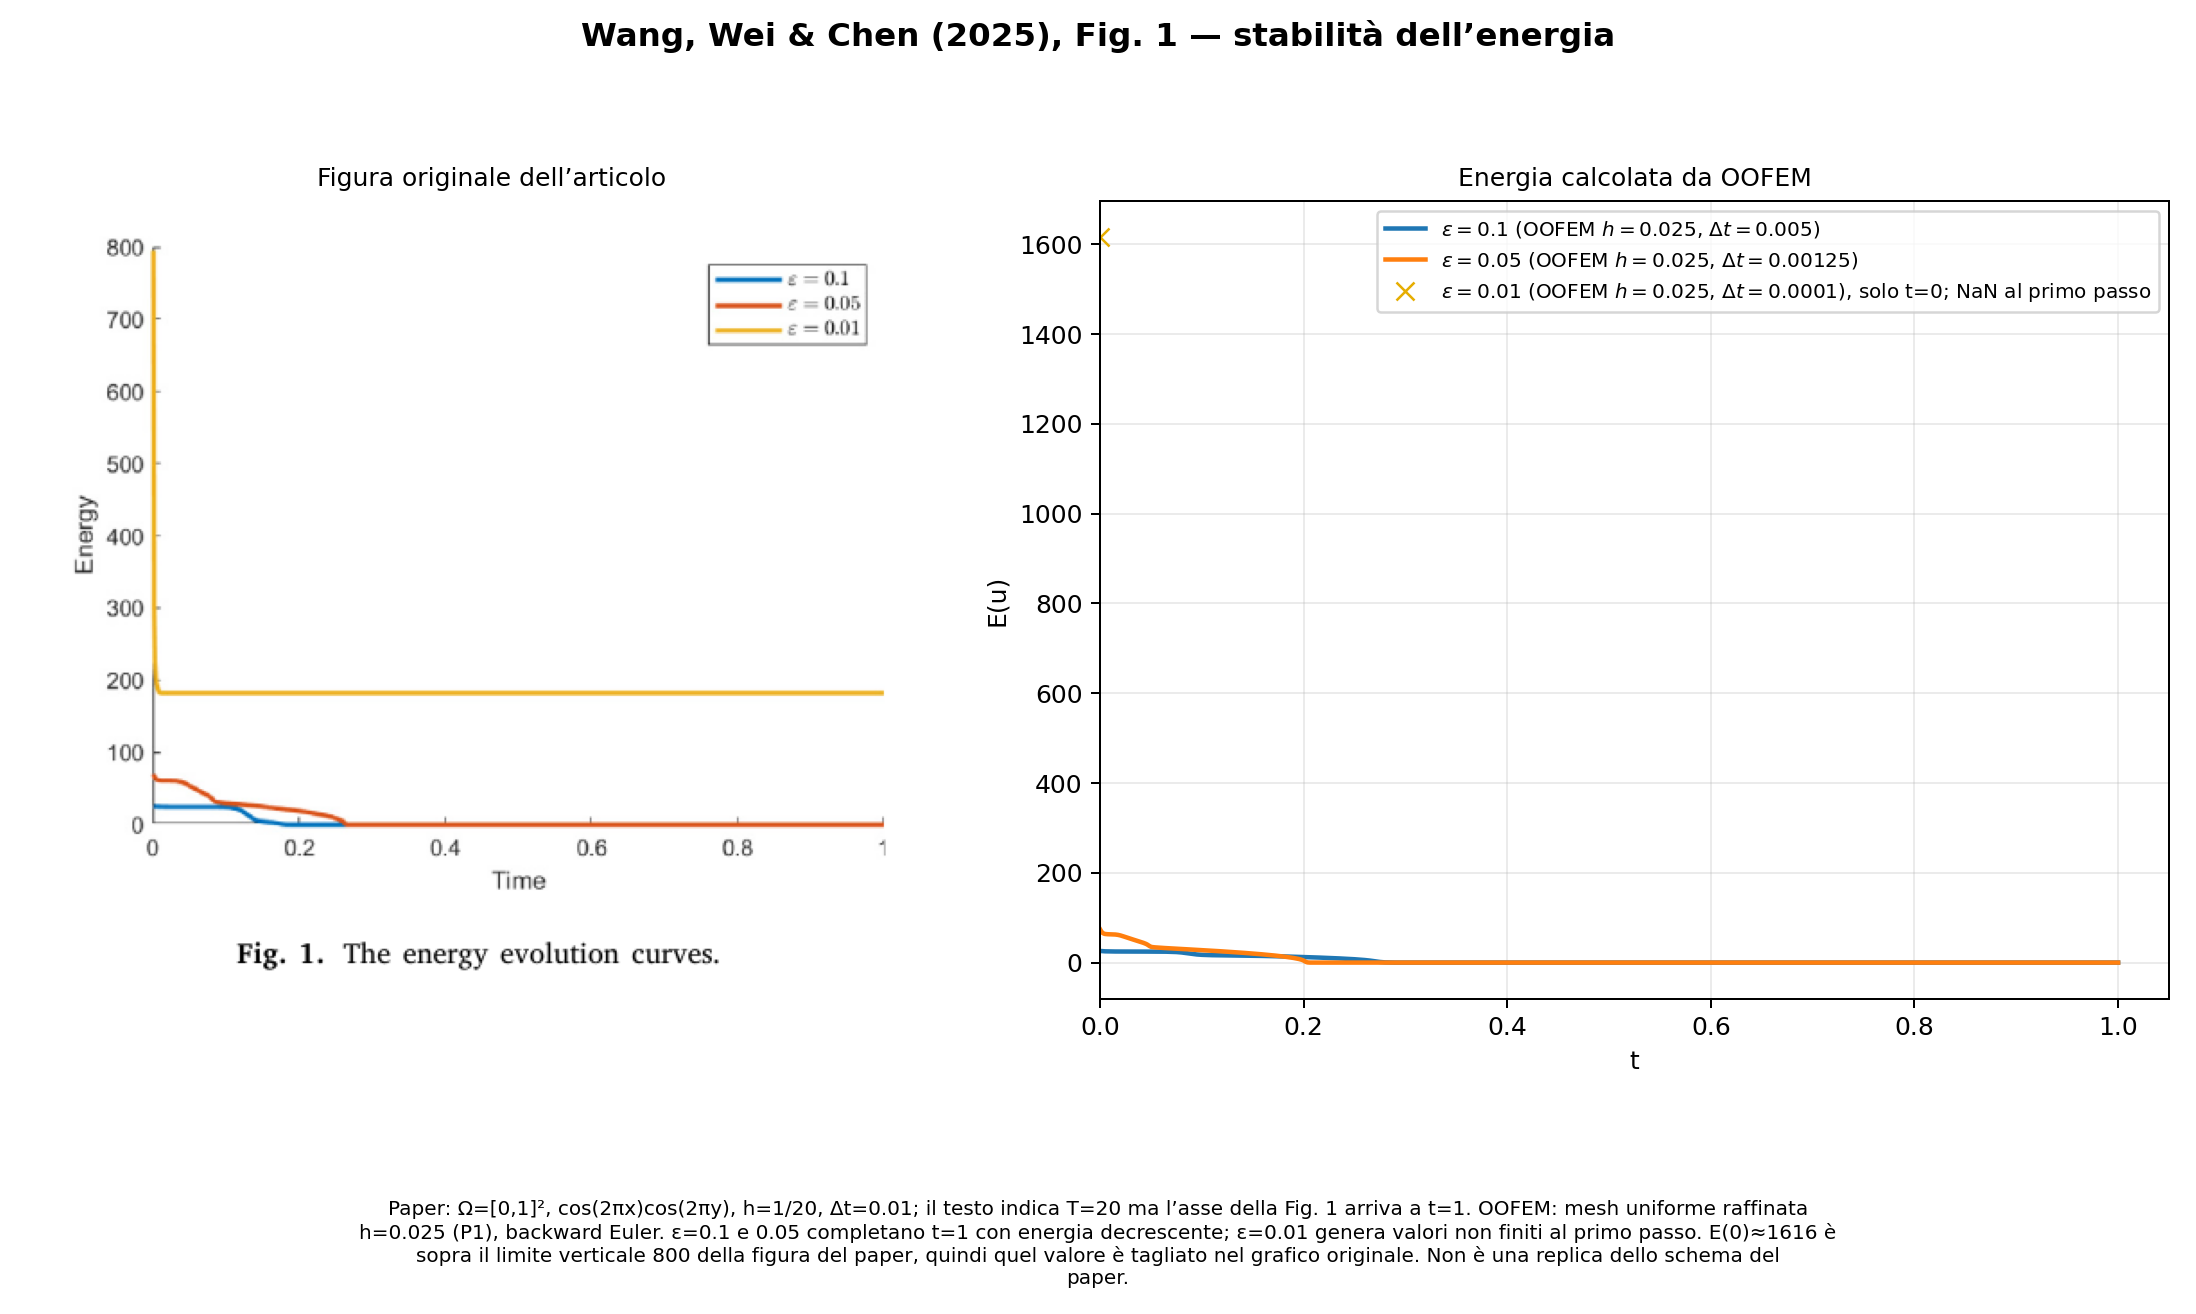
\includegraphics[width=\textwidth]{allen_cahn_paper_cases/figures/wang_figure1_comparison.png}
\end{center}
OOFEM usa backward Euler e la mesh raffinata \(h=0.025\); il paper usa \(h=0.05\) e uno schema diverso con stabilità energetica. Con i passi temporali precedenti, \(\varepsilon=0.1\) e \(0.05\) completano l’intervallo visibile fino a \(t=1\), con energia monotona e finale quasi nullo. Per \(\varepsilon=0.01\), i valori diventano non finiti al primo passo \(t=10^{-4}\): non c’è una curva valida oltre il punto iniziale. Il raffinamento non risolve questo problema. Il testo dichiara \(T=20\), mentre l’asse della figura termina a \(t=1\).
La mesh raffinata dà \(E(0)\simeq1615.9\) per \(\varepsilon=0.01\). La figura del paper ha l’asse verticale limitato a 800 e la curva tocca il bordo superiore: il valore iniziale è quindi fuori scala, non un riferimento leggibile pari a 800. Non abbiamo evidenza di una discrepanza nell’energia iniziale da questo grafico.

\clearpage
\subsection*{Akrivis e Li (2022), Figura 3}
\begin{center}
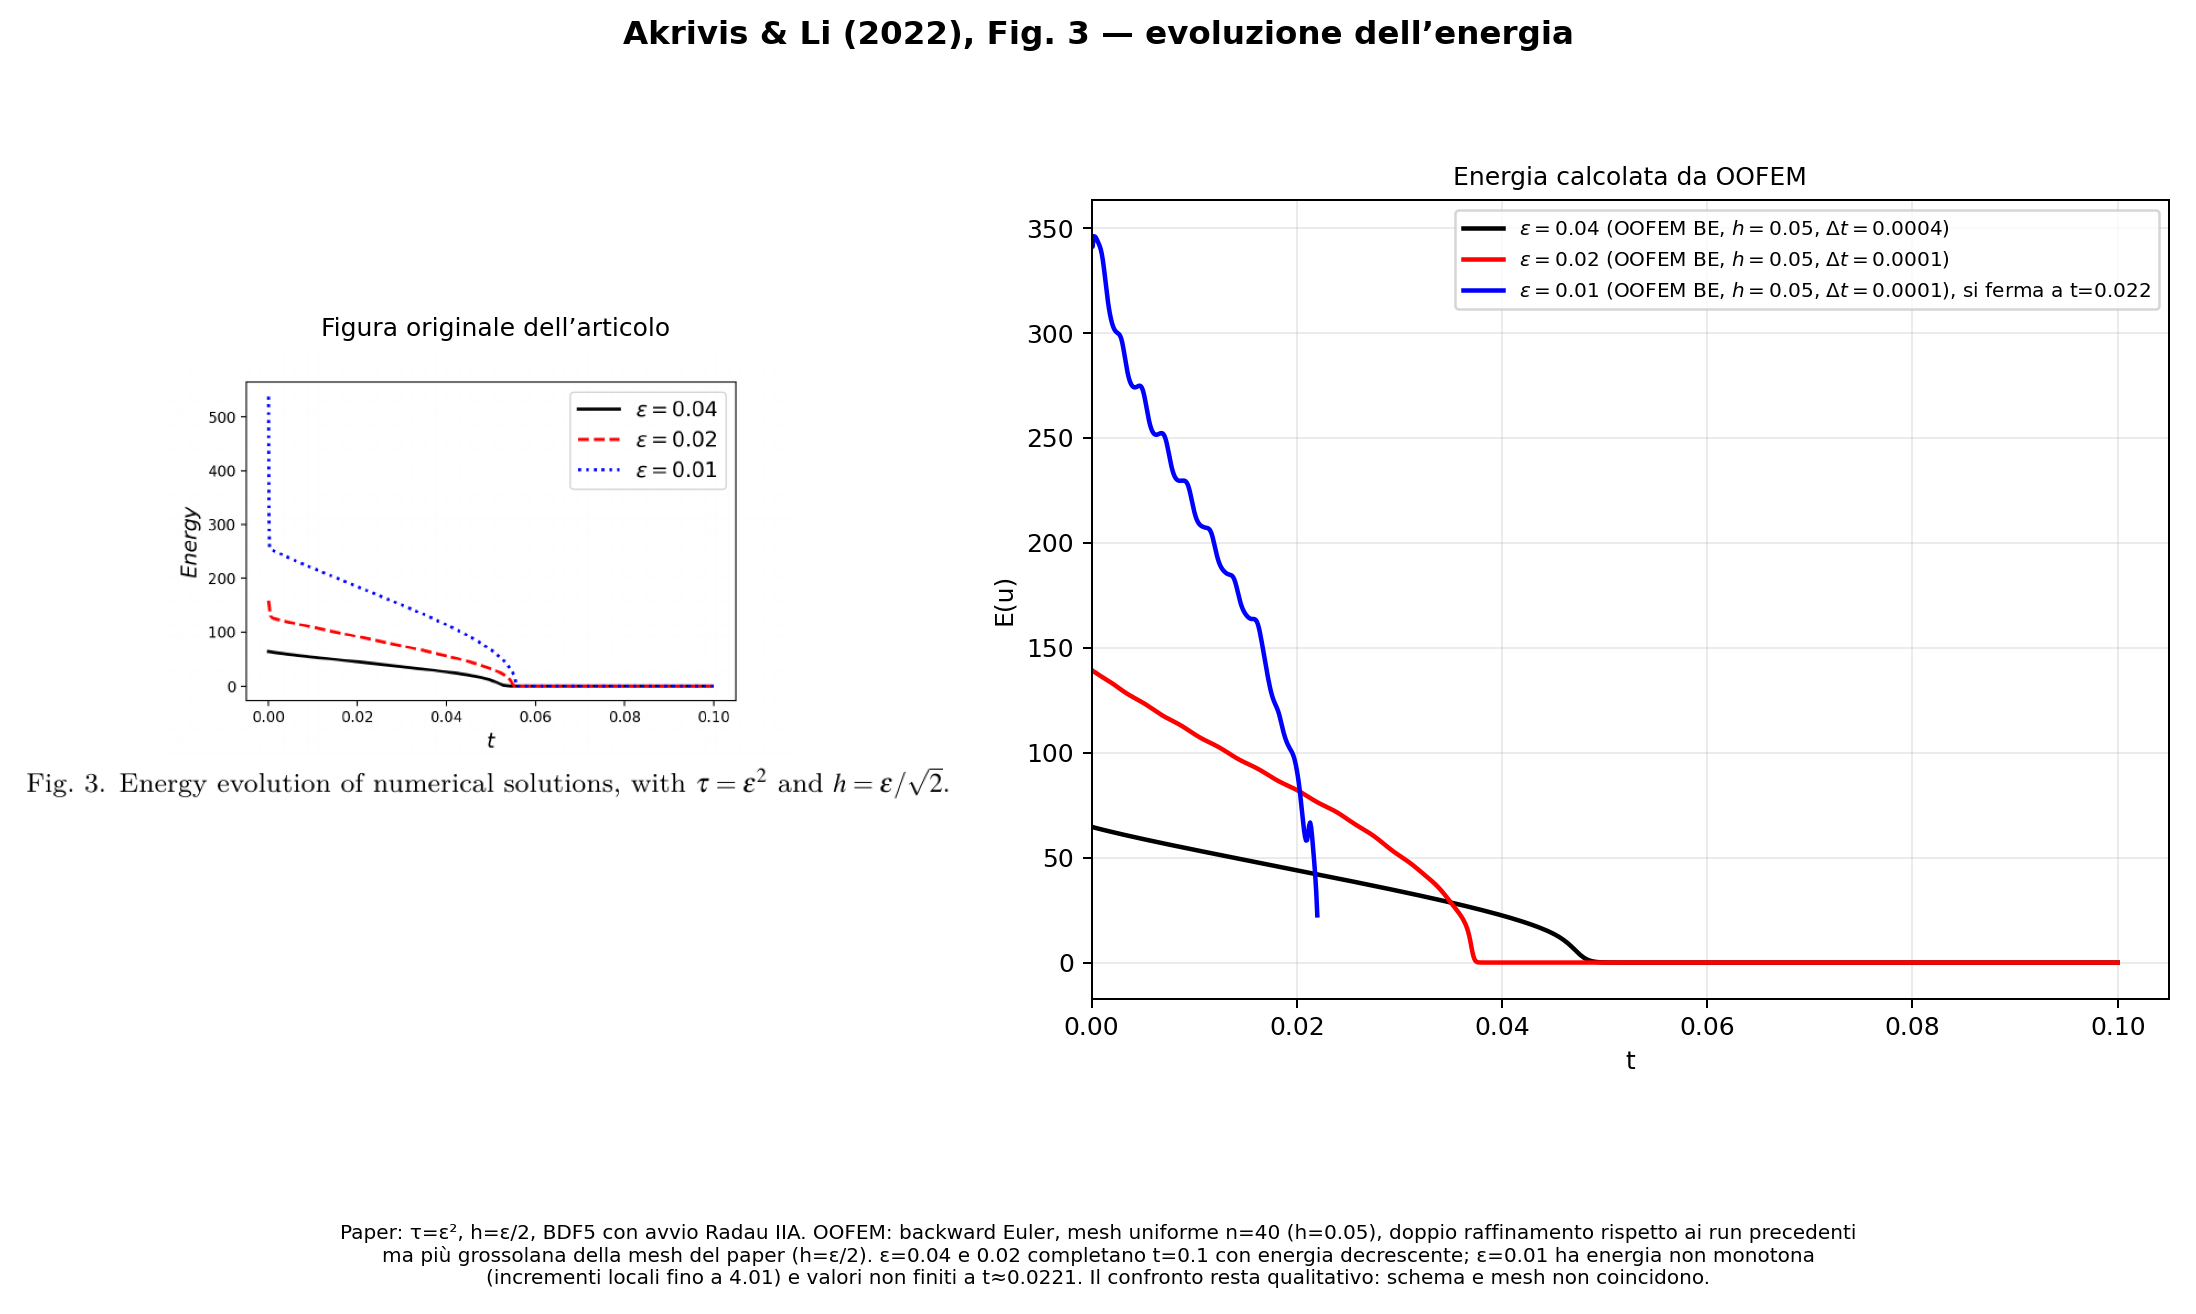
\includegraphics[width=\textwidth]{allen_cahn_paper_cases/figures/akrivis_figure3_comparison.png}
\end{center}
Il paper usa BDF5, avvio Radau IIA e \(h=\varepsilon/2\). OOFEM usa backward Euler su griglia uniforme \(h=0.05\), più grossolana del paper: il paper usa rispettivamente h=0.02, 0.01 e 0.005 per epsilon=0.04, 0.02 e 0.01. I casi \(\varepsilon=0.04\) e \(0.02\) completano \(t=0.1\) con energia monotona fino a valori prossimi a zero. Per \(\varepsilon=0.01\), l’energia non è monotona (incrementi locali fino a 4.01) e diventa non finita a \(t\simeq0.0221\); la curva è valida solo fino a circa \(t=0.022\). L’energia iniziale scende da circa 550 sulla mesh precedente a 346 sulla mesh raffinata, ma il run resta invalido.

\begin{center}\small
\begin{tabular}{l r l}
\toprule
Caso & \(h\) OOFEM & Esito del run raffinato \\
\midrule
Wang, \(\varepsilon=0.1\) & 0.025 & finito fino a \(t=1\), energia decrescente \\
Wang, \(\varepsilon=0.05\) & 0.025 & finito fino a \(t=1\), energia decrescente \\
Wang, \(\varepsilon=0.01\) & 0.025 & non finito al primo passo \(t=10^{-4}\) \\
Akrivis--Li, \(\varepsilon=0.04\) & 0.05 & finito fino a \(t=0.1\), energia decrescente \\
Akrivis--Li, \(\varepsilon=0.02\) & 0.05 & finito fino a \(t=0.1\), energia decrescente \\
Akrivis--Li, \(\varepsilon=0.01\) & 0.05 & energia non monotona; non finito a \(t\simeq0.0221\) \\
\bottomrule
\end{tabular}
\end{center}
Il raffinamento migliora la risoluzione, ma il confronto non è quantitativo: gli schemi temporali restano diversi e Akrivis--Li richiede \(h=\varepsilon/2\). Per \(\varepsilon=0.01\) persiste la non-finitezza.

\clearpage
\section{Stato e prossimi controlli}
\begin{itemize}
 \item Build Debug riuscita; \texttt{ctest -R allencahn}: 6/6 test passati, incluso il nuovo MMS sinusoidale.
 \item Per Wang et al. gli ordini spaziali sono corretti; i valori L2 e il raffinamento simultaneo non coincidono ancora con il paper.
\item Per Akrivis--Li è stato aggiunto il BDF di ordine 1--5 con passo fisso; i casi Fig. 3 con $\varepsilon=0.04$ e $0.02$, mesh $h=\varepsilon/2$ e Newton completo sono terminati. L’avvio automatico BDF1--BDF5 non coincide ancora con i quattro passi iniziali Radau IIA a tre stadi del paper.
\item La mesh pubblicata dagli articoli è descritta tramite passo/regolarità ma non sono forniti i nodi e la connettività; OOFEM usa quindi triangoli uniformi con gli stessi $h$, non una replica della topologia originale. Per Wang resta inoltre da implementare la formulazione accoppiata P1 $(\phi_h,u_h)$.
 \item Sono pronti gli input Wang Fig. 1 con $h=1/20$ e $\Delta t=0.01$. Il run BE standard converge per $\varepsilon=0.1$ con Newton completo, ma per $\varepsilon=0.05$ non converge al passo 7: serve la formulazione accoppiata del paper per riprodurne la stabilità.
 \item Stato run (22 ottobre 2026): Akrivis--Li $\varepsilon=0.04$ e $0.02$ completati rispettivamente a $t=0.1008$ e $0.1$; Wang $\varepsilon=0.1$ completato; Wang $\varepsilon=0.05$ fallito al passo 7 per mancata convergenza. Akrivis--Li $\varepsilon=0.01$ con $h=0.005$, $\tau=10^{-4}$ e BDF5 convergeva fino al passo 17/1000, poi è stato fermato: il solver diretto richiede circa 22 s per passo. PETSc non è configurabile perché manca \texttt{mpi.h}; l’installazione degli header MPI è stata negata dal sistema. Questo caso resta incompleto.
\item Nessuno dei due articoli considera il bordo dinamico del progetto. I casi analizzati riguardano il bulk, e i confronti attuali non bastano a dichiarare il codice pienamente validato.
\end{itemize}

Gli input originali e gli script di raffinamento/confronto sono in \path{doc/allen_cahn_paper_cases/}; input e campi VTK dei nuovi run sono in \path{/tmp/ac_refined/}. I run precedenti restano in \path{/tmp/ac_paperplots/}; i run MMS sono in \path{/tmp/ac_paper1/} e \path{/tmp/ac_paper2/}. Il sorgente Markdown è \path{doc/Confronto_articoli_AllenCahn_IT.md}.

\end{document}
